\documentclass[11pt]{article}
\usepackage[margin=1in]{geometry}
\usepackage{amsmath}
\usepackage{graphicx}
\usepackage{enumitem}
\usepackage{tcolorbox}
\usepackage{fancyhdr}
\usepackage{tikz}

% Header setup
\pagestyle{fancy}
\fancyhf{}
\lhead{AP Statistics - Unit 2, Lesson 4}
\rhead{Name: \underline{\hspace{3cm}}}
\cfoot{\thepage}

\title{\textbf{Sentence Frame Worksheet\\
Explanatory vs. Response Variables \& Scatter Plots\\
\large Unit 2, Lesson 4 - Video 1}}
\date{}

\begin{document}
\maketitle
\thispagestyle{fancy}

\section*{Learning Objectives}
As you watch the video, complete these learning objectives:
\begin{enumerate}
    \item For bivariate data, I will learn how to determine which variable is the \underline{\hspace{3cm}} variable.
    \item I will learn how to determine which variable is the \underline{\hspace{3cm}} variable.
    \item I will learn how to construct a \underline{\hspace{3cm}}.
\end{enumerate}

\section*{Part 1: Context - The Income Achievement Gap}

\subsection*{The Problem}
In the United States, \underline{\hspace{2cm}} and \underline{\hspace{2cm}} income students tend to perform better on math exams than \underline{\hspace{2cm}} income students on average. This phenomenon is called the \underline{\hspace{4cm}}.

\subsection*{Important Notes About the Data}
\begin{tcolorbox}[colback=yellow!10!white,colframe=red!50!black]
Complete these critical understanding points:
\begin{itemize}
    \item This data says nothing about \underline{\hspace{3cm}} performance.
    \item The data represents trends of \underline{\hspace{2cm}} for full groups.
    \item This data says nothing about \underline{\hspace{3cm}} intelligence.
\end{itemize}
\end{tcolorbox}

\subsection*{Factors to Consider}
\begin{enumerate}
    \item \textbf{Wealth Privilege:} Middle and upper income students often don't face as many \underline{\hspace{3cm}} as their lower income peers.
    
    \item \textbf{Income Attendance Gap:} Higher income areas tend to have \underline{\hspace{2cm}} chronically absent students.
    
    Possible reasons include:
    \begin{itemize}
        \item Better \underline{\hspace{3cm}} access
        \item Less need to \underline{\hspace{2cm}} to support family
    \end{itemize}
\end{enumerate}

\section*{Part 2: The Hypothesis}

Some school systems believe: ``\underline{\hspace{3cm}} is the key to raise test scores for lower income students.''

Their logic: If poverty causes low attendance, then by making attendance \underline{\hspace{2cm}} through systems and policies, we might see \underline{\hspace{2cm}} test scores.

\textbf{Today's Question:} Is this statement reasonable or is it ``BS''? 
\begin{tcolorbox}[colback=blue!10!white,colframe=blue!50!black]
Note: BS stands for \underline{\hspace{3cm}}
\end{tcolorbox}

\section*{Part 3: Analyzing the Data}

\subsection*{The Data Set}
We have a random sample of \underline{\hspace{1cm}} students with two measurements:
\begin{enumerate}
    \item Percent of \underline{\hspace{3cm}} each student attended
    \item Number of \underline{\hspace{3cm}} answered correctly on the Texas end-of-year Algebra 1 assessment
\end{enumerate}

\subsection*{Identifying Variable Types}
Complete the classification:

\begin{center}
\begin{tabular}{|l|c|c|}
\hline
\textbf{Variable} & \textbf{Type (Explanatory/Response)} & \textbf{Symbol (X or Y)} \\
\hline
Attendance (\%) & \underline{\hspace{3cm}} & \underline{\hspace{1.5cm}} \\
\hline
Questions Correct & \underline{\hspace{3cm}} & \underline{\hspace{1.5cm}} \\
\hline
\end{tabular}
\end{center}

\textbf{Memory Tip:} The \underline{\hspace{1cm}} variable is explanatory (they both start with the same letter!).

\subsection*{Why These Classifications?}
We think attendance might \underline{\hspace{2cm}} student performance on the test, so:
\begin{itemize}
    \item Attendance is the \underline{\hspace{3cm}} variable (it explains)
    \item Test performance is the \underline{\hspace{3cm}} variable (it responds)
\end{itemize}

\section*{Part 4: Creating the Visualization}

\subsection*{Choosing the Right Plot}
Answer these questions to determine the appropriate visualization:

\begin{enumerate}
    \item How many variables are being measured? \underline{\hspace{1cm}}
    \item Are these variables categorical or quantitative? \underline{\hspace{3cm}}
    \item Why are they this type? Because each variable is \underline{\hspace{3cm}} with an inherent \underline{\hspace{2cm}} to it.
\end{enumerate}

\textbf{Conclusion:} When we have two \underline{\hspace{3cm}} variables, we should make a \underline{\hspace{3cm}}.

\subsection*{Essential Components of a Scatter Plot}
\begin{tcolorbox}[colback=green!10!white,colframe=green!50!black]
\textbf{When creating a scatter plot, you MUST include:}
\begin{enumerate}
    \item A \underline{\hspace{2cm}} that describes the \underline{\hspace{2cm}}
    \item \underline{\hspace{2cm}} labeled with each variable showing:
    \begin{itemize}
        \item Which is \underline{\hspace{3cm}} (on x-axis)
        \item Which is \underline{\hspace{3cm}} (on y-axis)
    \end{itemize}
    \item \underline{\hspace{2cm}} with \underline{\hspace{2.5cm}} to show exactly what scale you're using
\end{enumerate}
\end{tcolorbox}

\subsection*{Understanding the Plot}
In a scatter plot:
\begin{itemize}
    \item Each individual is represented as a set of \underline{\hspace{3cm}}
    \item The x-coordinate represents the \underline{\hspace{3cm}} variable
    \item The y-coordinate represents the \underline{\hspace{3cm}} variable
\end{itemize}

\section*{Part 5: Practice Space}
Draw and label a scatter plot with proper components:

\begin{center}
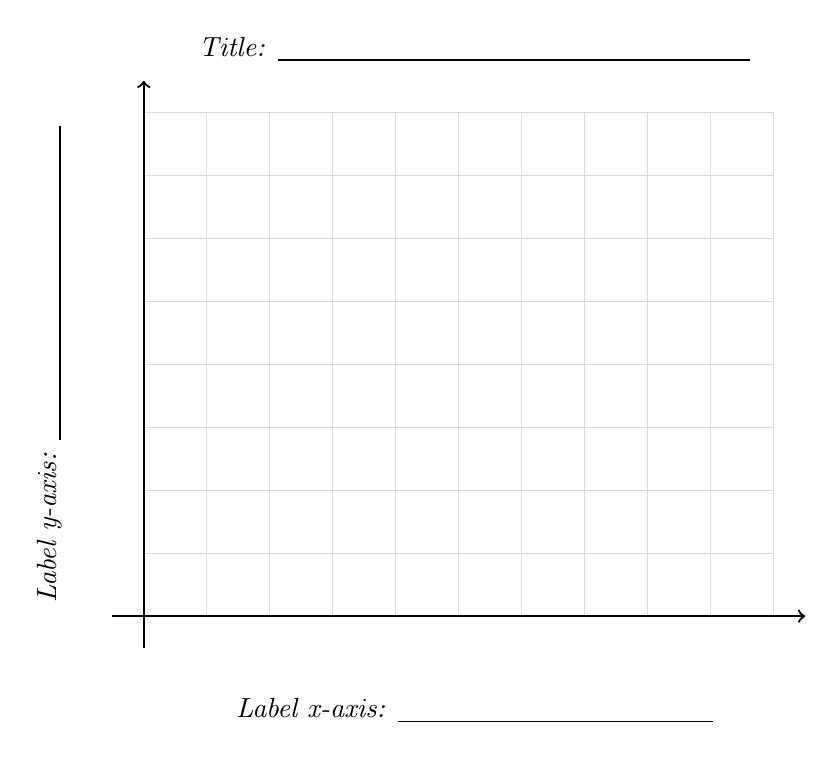
\begin{tikzpicture}[scale=0.8]
    % Grid
    \draw[very thin, gray!30] (0,0) grid (10,8);
    
    % Axes
    \draw[thick,->] (-0.5,0) -- (10.5,0);
    \draw[thick,->] (0,-0.5) -- (0,8.5);
    
    % Labels placeholders
    \node at (5.25,-1.5) {\textit{Label x-axis: \underline{\hspace{4cm}}}};
    \node[rotate=90] at (-1.5,4) {\textit{Label y-axis: \underline{\hspace{4cm}}}};
    \node at (5.25,9) {\textit{Title: \underline{\hspace{6cm}}}};
\end{tikzpicture}
\end{center}

\section*{Key Takeaways}
Complete these summary statements:

\begin{enumerate}
    \item \underline{\hspace{3cm}} variables predict or explain trends in \underline{\hspace{3cm}} variables.
    
    \item Scatter plots visualize trends between \underline{\hspace{1cm}} quantitative variables.
    
    \item When making a scatter plot, always include:
    \begin{itemize}
        \item A \underline{\hspace{2cm}}
        \item \underline{\hspace{2cm}} axes (with units if applicable)
        \item Properly shown \underline{\hspace{2cm}} with tick marks
    \end{itemize}
\end{enumerate}

\section*{The Statistician's Motto}
When analyzing data, Mr. Young Saver reminds us to be:
\begin{enumerate}
    \item Be \underline{\hspace{2.5cm}}
    \item Be \underline{\hspace{2.5cm}}
    \item Be \underline{\hspace{2.5cm}}
    \item And avoid \underline{\hspace{1.5cm}} at all costs!
\end{enumerate}

\section*{Looking Ahead}
\begin{tcolorbox}[colback=orange!10!white,colframe=orange!50!black]
\textbf{Next Video Question:} How would you describe the \underline{\hspace{2cm}} that you see in a scatter plot?
\end{tcolorbox}

\vspace{1cm}

\section*{Reflection Questions}
\begin{enumerate}
    \item Why is it important that the data about test scores reflects averages and not individual performance?
    
    \vspace{2cm}
    
    \item In your own words, explain the difference between an explanatory and a response variable:
    
    \vspace{3cm}
    
    \item Why might it be problematic to assume that simply increasing attendance will automatically improve test scores?
    
    \vspace{3cm}
\end{enumerate}

\end{document}